\hypertarget{modelview_8cpp}{}\section{Файл Projects/labs/course\+\_\+project\+\_\+cg/src/widgets/modelview.cpp}
\label{modelview_8cpp}\index{Projects/labs/course\+\_\+project\+\_\+cg/src/widgets/modelview.\+cpp@{Projects/labs/course\+\_\+project\+\_\+cg/src/widgets/modelview.\+cpp}}
{\ttfamily \#include \char`\"{}modelview.\+h\char`\"{}}\\*
{\ttfamily \#include $<$Q\+Style$>$}\\*
{\ttfamily \#include \char`\"{}src/animation/rotatetransformation.\+h\char`\"{}}\\*
{\ttfamily \#include \char`\"{}src/animation/scene.\+h\char`\"{}}\\*
{\ttfamily \#include \char`\"{}src/animation/renderer.\+h\char`\"{}}\\*
{\ttfamily \#include \char`\"{}src/animation/sceneobjectfactory.\+h\char`\"{}}\\*
{\ttfamily \#include \char`\"{}src/animation/lightzbufferrenderer.\+h\char`\"{}}\\*
{\ttfamily \#include \char`\"{}src/animation/objloader.\+h\char`\"{}}\\*
Граф включаемых заголовочных файлов для modelview.\+cpp\+:\nopagebreak
\begin{figure}[H]
\begin{center}
\leavevmode
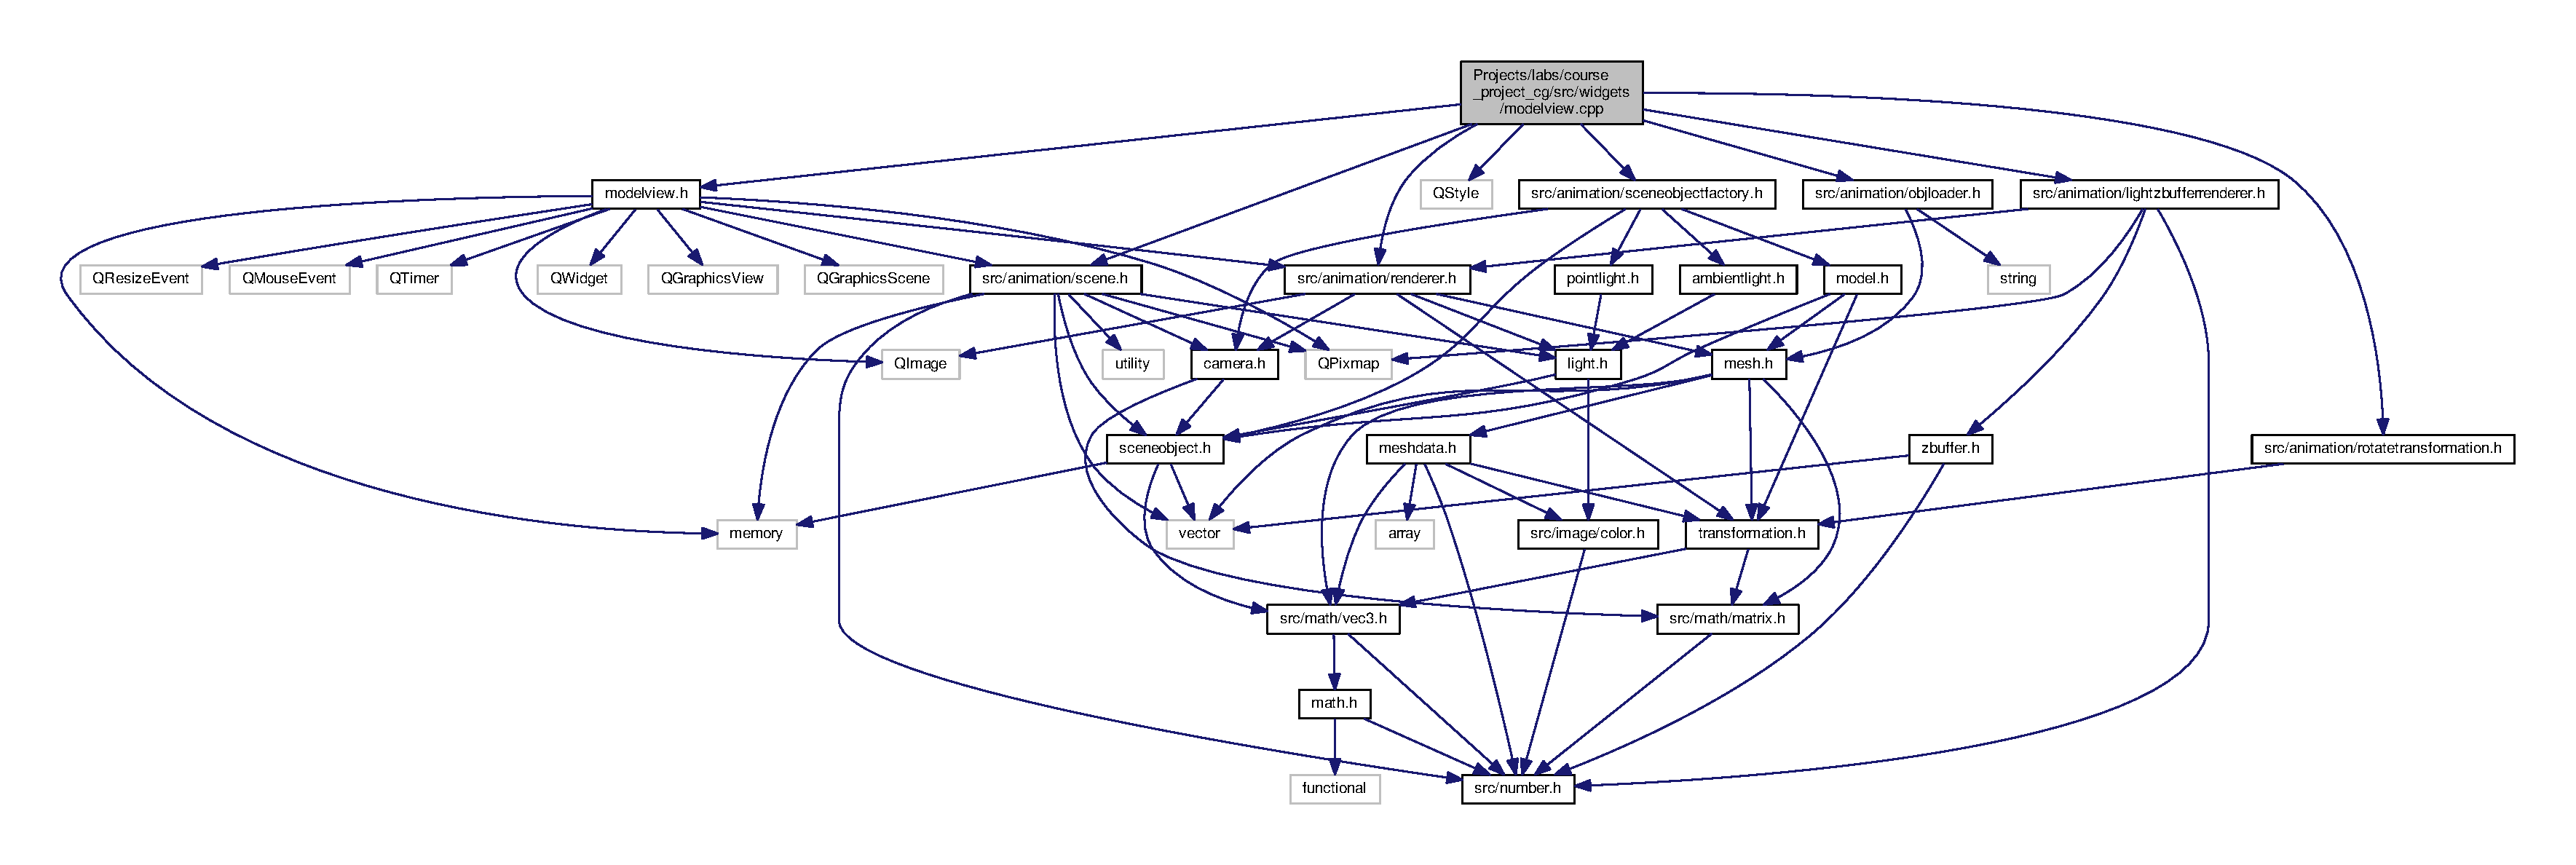
\includegraphics[width=350pt]{d1/d1b/modelview_8cpp__incl}
\end{center}
\end{figure}
